\documentclass{article}

\usepackage{booktabs}
\usepackage{tabularx}
\usepackage{color}
\usepackage{xcolor}
\usepackage{hyperref}
\usepackage[normalem]{ulem}
\usepackage{graphicx}

\title{SE 3XA3: Development Plan\\OpenCameraRefined}

\author{Team 211, Team Elon
		\\ Pedram Yazdinia, yazdinip
		\\ Zayed Sheet, sheetz
		\\ Faisal Jaffer, jaffem1
		\\ Dominik Buszowiecki, buszowid 
}

\date{\today}

%\input{../Comments}

\begin{document}

\begin{table}[hp]
\caption{Revision History} \label{TblRevisionHistory}
\begin{tabularx}{\textwidth}{llX}
\toprule
\textbf{Date} & \textbf{Developer(s)} & \textbf{Change}\\
\midrule
1/31/2020 & Pedram Yazdinia, Zayed Sheet & Initial Document (Rev0)\\
4/4/2020 & Pedram Yazdinia & Revision 1\\
\bottomrule
\end{tabularx}
\end{table}

\newpage

\maketitle


This document contains the development plan for the implementation of ''OpenCamera”. The intent of this document is to set appropriate meeting times and a working communication plan that is feasible to all members of the group. It also set the styles standards by which the code shall be written and pushed to git. Each member is assigned a role and tasks that they must complete and update the progress to the team in the weekly set meetings.


\section{Team Meeting Plan}

In addition to the lab times where all members do tutorial work and improve the project, each group member is responsible for consistent presence in weekly online and personal meetings. These meetings take place every Monday and Saturday with different purposes. Saturday meetings take place \textcolor{red}{at 8 pm }to bring every person of the group up to date while evaluating the progress done over the week. These meetings are brief and take place over online platforms(Facebook Messenger). Monday meetings take place \textcolor{red}{at 5 pm } to provide a chance for the developers to discuss, design and implement on any aspect of the product. It is very crucial that developers personally attend these meetings. These meetings usually take around an hour, within study rooms of Thode Library. Within the group, Zayed Sheet will take control over the structure of each agenda as the group chair. He will ensure that the meeting flows as planned through agenda and that each member is informed of their “homework”. Finally, he is responsible for gathering the written statement of the decisions made. 

\section{Team Communication Plan}

In order to ensure all members are up to date with the project, the team will be communicating through a Facebook Messenger group. Whenever a team member decides to work on a portion of the project, they will be required to inform the group about what they are about to do. This is to ensure that there are no conflicts or overlap between the work done among group members. The messenger group will also be used to plan meetings or inform the others if they cannot make the meetings.

\section{Team Member Roles}

\begin{table}[h]
\begin{tabular}{|l|l|}
\hline
\textbf{Group Member} & \textbf{Role}                   \\ \hline
Pedram Yazdinia       & Git expert, LaTex expert        \\ \hline
Dominik Buszowiecki   & Java Expert, Latex expert       \\ \hline
Faisal Jaffer         & Group Leader, Java Expert       \\ \hline
Zayed Sheet           & Tensorflow expert, Latex expert \\ \hline
\end{tabular}
\end{table}
\section{Git Workflow Plan}

The original open source project will be cloned as OpenCameraRefined in GitLab. Since our team has a single important feature, will use the Feature Branch workflow to maintain our codebase on Git. Each member will work on the same branch, solving different issues that need to be addressed. Each commit is going to be assigned a solution label that targets the problem that it has addressed. When the feature has been implemented on the branch, it will be merged into the master branch.
\section{Proof of Concept Demonstration Plan}

The proof of concept will surely be one of the most stressful parts of the assignment, however with proper planning and preparation we can minimize any risks or unexpected events. 

The addition of a picture auto capture feature will be risky because of the machine learning models that will need to be implemented for it to work. The plan to demonstrate the feasibility of this feature is to show a working concept of a machine learning model that can successfully distinguish between different gestures. This does not have to be directly incorporated in the app at this stage.

Because our app runs on a separate environment it will require android studio. Integration between the Java code and the android platform will need to be experimented a week in advance to ensure familiarity within the environment. We will use Zayed Sheet’s android mobile device to experiment with the environment and demonstrate the proof of concept. 

Lastly, testing will be a vital component to ensure the smoothness of the demonstration. We will use unit testing software such as JUnit version 5 for a more efficient process. In addition, we will use the android studio Emulator to test features wherever possible, in order to reduce the time for switching between environments. 


\section{Technology}

The application will be written using Java with the Android Studio IDE. Android Studio will be used as it features a built in device emulator to allow testing to be performed on various devices and android versions. On top of this, we plan to test the application a real device which is another feature that Android Studio offers. In order to produce documentation, the IDE includes a built in JavaDoc generator which will read the JavaDoc comments that our team will have written in the code. \textcolor{red}{Finally, for Machine Learning applications used to detect gestures, the team has decided to use Google's Brain Team services, mainly the Tensor Flow library. It allows for training of a specific model which will then be used along with Android Neural Networks API to provide proper gesture recognition on the trained object.}

\section{Coding Style}

Consistency between coding styles throughout the project is important in order for all group members to be able to revise and review other group member’s code. This is why all our project code will follow the “Google Java Style Guide”

\section{Project Schedule}

\begin{figure}[h!]
\centering
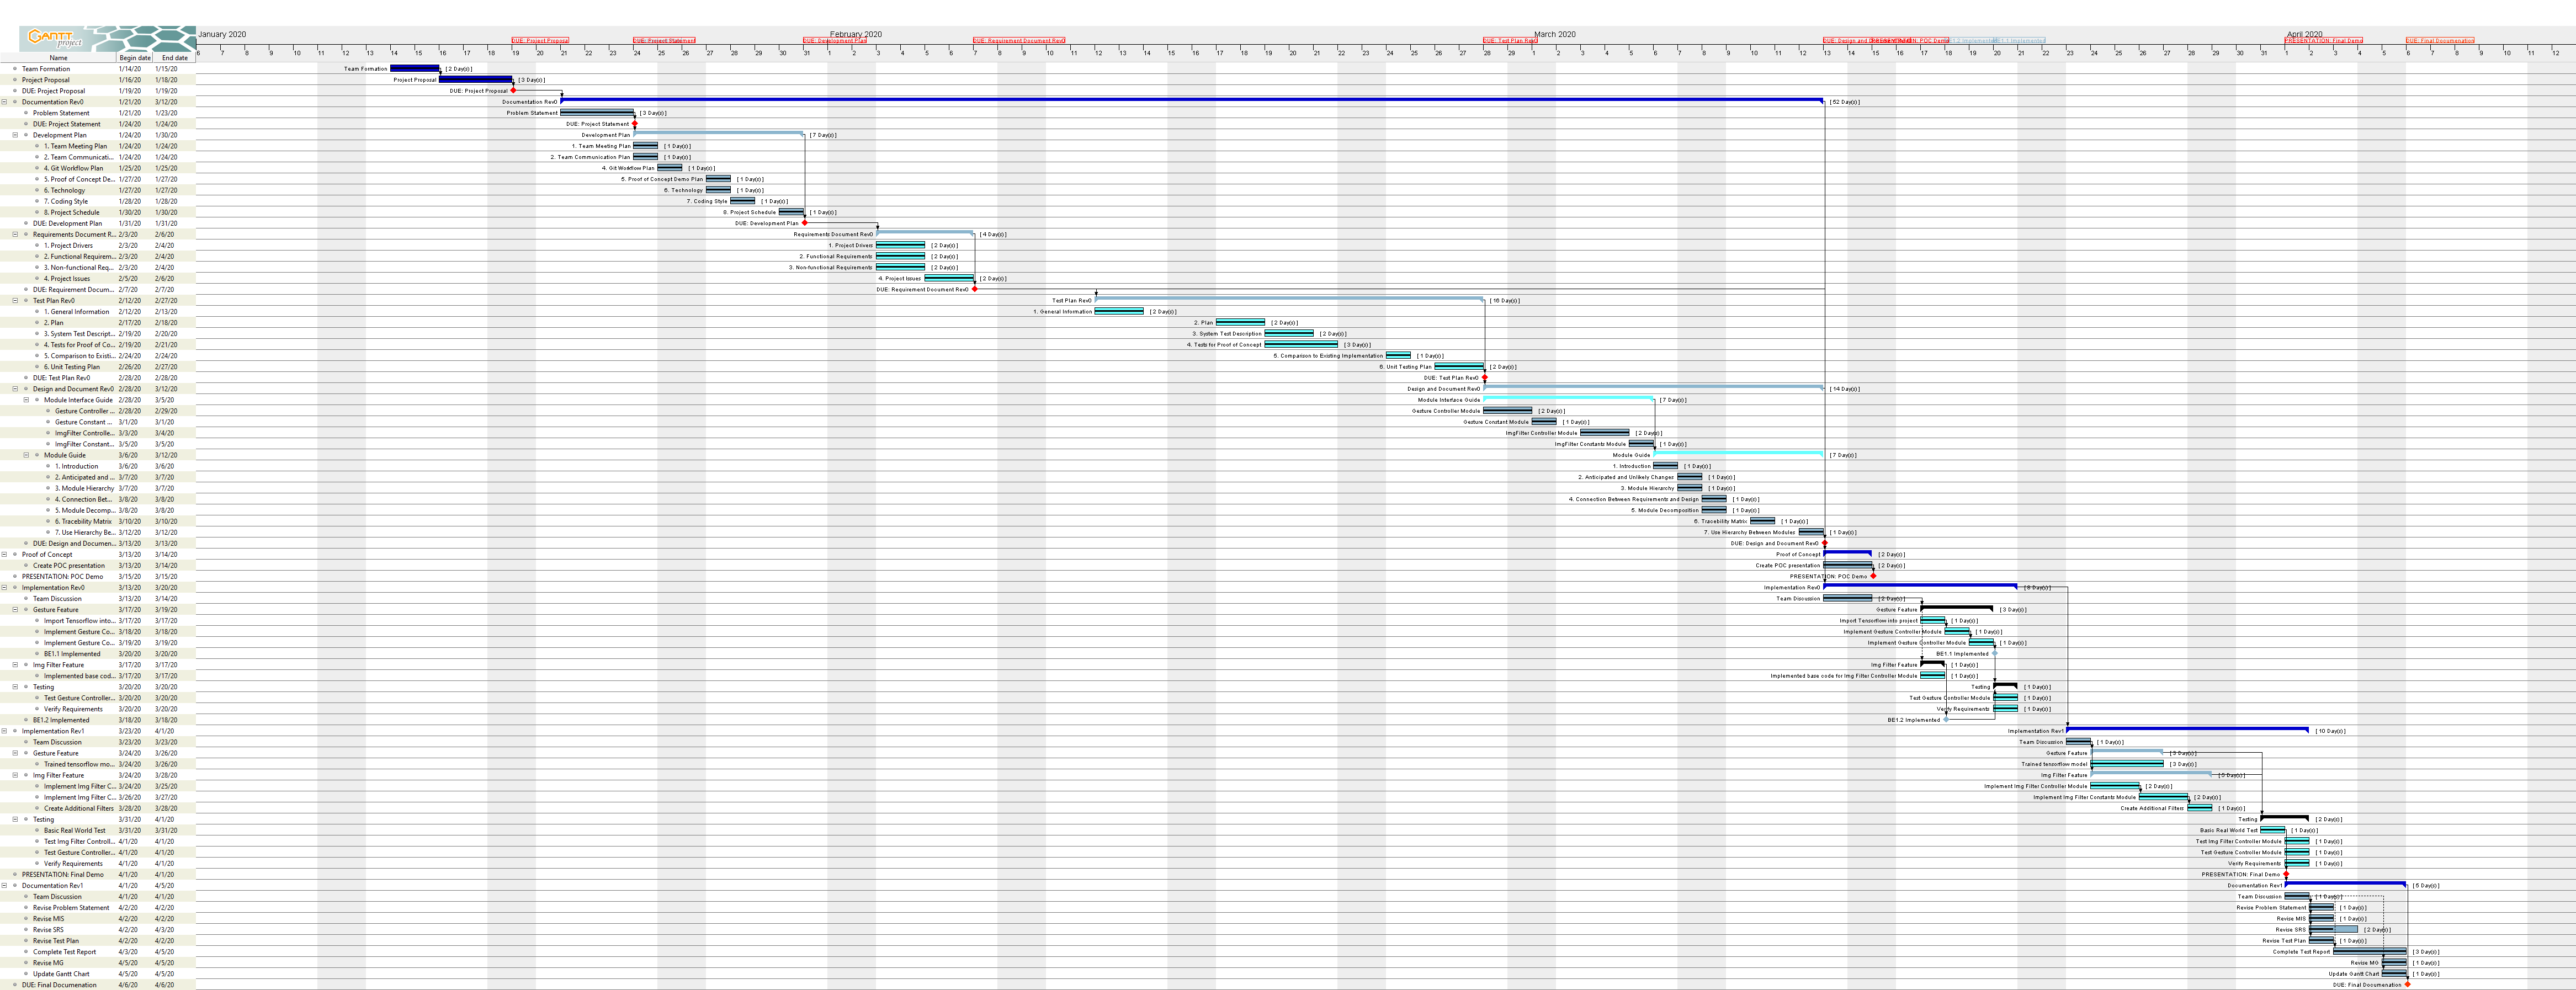
\includegraphics[width=100mm, scale = 2]{GanttChart}
\caption{GanttChart}
\label{fig:method}
\end{figure}
Further information and details can be found within the \href{https://gitlab.cas.mcmaster.ca/yazdinip/opencamerarefined/-/blob/master/ProjectSchedule/Gantt.pdf}{Gantt Chart}.

\section{Project Review}
{\color{red}
The project development finished on April 3rd 2020, and the team had a chance to review and reflect on the work done. In our mind, the project was a success. We set out to create an application that in its core combines the stock Android Camera applications with the popular functionalities of mainstream social media applications such as Instagram and Snapchat; and we believe that we achieved our goal. Nevertheless, the project was less than we hoped and imagined. One of our weaknesses came back to the fact that many of us underestimated the scope of the original project. Since the project was not very new, there was a lot of time-consuming configuration just to get the application running on the latest frameworks. In addition, the model training requires a very large database of pictures of specific gestures until it can look stable as seen on many other applications. The pictures had to be manually taken and even then, each picture had to be prepared before being processed by the Google services. On the other hand, the original project was very complex. It consists of thousands of lines and hundreds of methods and classes with advanced architecture and shortcuts which were hard to understand. With all these tedious works that were not really part of the main development plan, the team fell behind of the schedule. However, we had our moments too. The team was able to communicate well to arrive at agreements when it came down to design decisions and since we were all very comfortable with each other, we easily asked for help. 

There are many ways to improve our process and development plan. In many areas, the team meetings didn’t go according to the plan. In the future, the team needs to allocate more time to the structure of the meetings. The meetings need to have more specific purposes and details as to how the meeting should flow. There should be more time allocated to defining the scope of the project within the team. Although we had a general structure given by the course, the code development needed to start sooner and given more time. Furthermore, the first few sessions should exclusively be allocated to creating a general, shared vision of the final product that everyone accepts. It is crucial that the team members are constantly on the same page, as it proved to be our biggest mistake.

}

\end{document}